\section{Fault-Tolerance Mechanisms}

\subsection{Timeouts}

\subsection{Bulkheads}

\subsection{Circuit Breaker}

\begin{figure}[H]
\centering
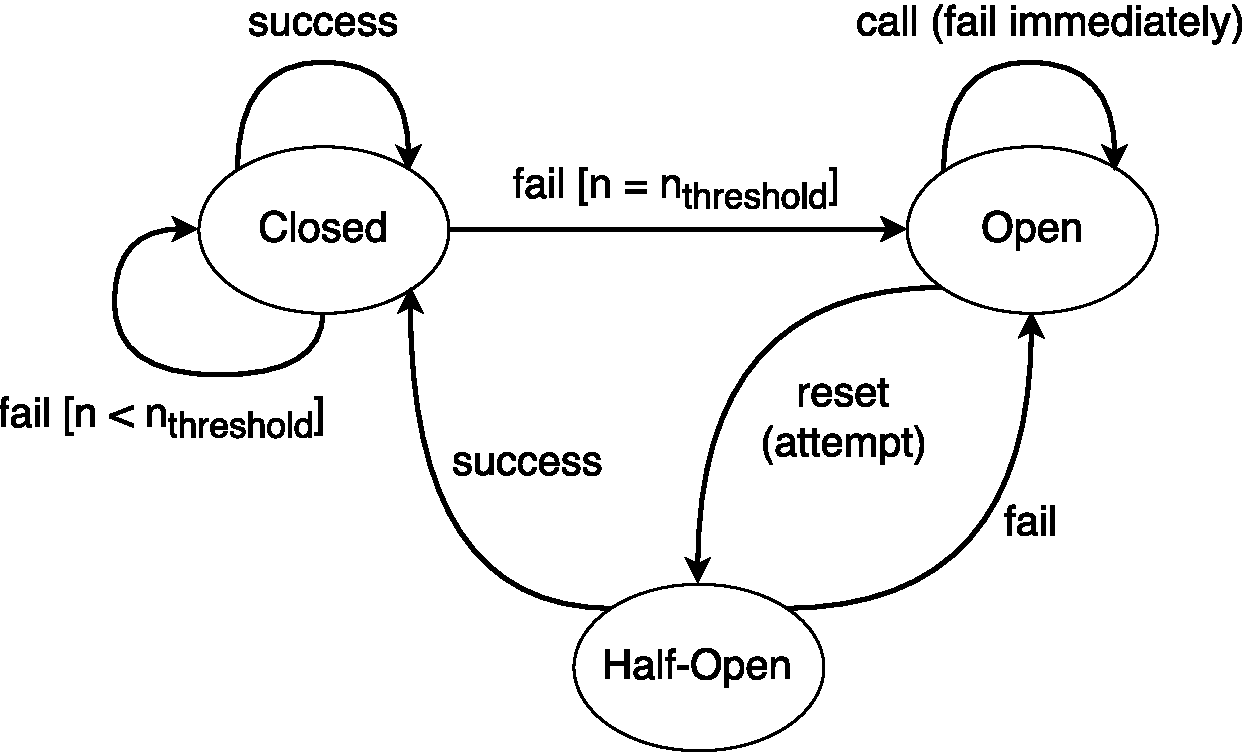
\includegraphics[width=\textwidth]{../media/CircuitBreakerState.pdf} 
\caption{State machine representing the \textit{Circuit Breaker} state. The
	circuit can be the states \textit{Closed}, \textit{Open} or 
	\textit{Half-Open}.}
\label{fig:circuitbreakerstate}
\end{figure}

\subsection{Replication}
% Replication of stateless services, split workload

\subsection{Redundancy}
% Multiple hosts and services ready for fail-over

\subsection{Resilience}
% Self healing of Docker Swarm orchestration

